\documentclass[10pt]{article}

\usepackage[a4paper,margin=0.72in]{geometry}
\usepackage{array}
\usepackage{booktabs}
\usepackage{caption}
\usepackage{float}
\usepackage{graphicx}
\usepackage{microtype}
\usepackage{pgfplots}
\usepackage{tikz}
\usepackage{titlesec}

\pgfplotsset{compat=1.18}
\captionsetup{font=small,aboveskip=3pt,belowskip=3pt}
\titleformat{\section}{\bfseries\large}{\thesection.}{0.45em}{}
\titlespacing*{\section}{0pt}{0.65em}{0.25em}
\setlength{\parskip}{0.25em}
\setlength{\parindent}{0pt}
\setlength{\tabcolsep}{4pt}

\title{\vspace{-1.3em}\bfseries Empirical Evidence of Operational Domain Shift}
\author{Angad Singh Ahuja}
\date{\vspace{-0.8em}June 6, 2026}

\begin{document}
\maketitle
\vspace{-1.4em}


\section{Annotated Data is Diverse and Operationally Detailed}

\begin{table}[H]
\centering
\caption{Baseline annotation numbers.}
\small
\begin{tabular}{lrrrrrr}
\toprule
Annotation file & Images & Boxes & Lamps & Poles & Confounders & Polygons\\
\midrule
zip001 & 100 & 336 & 244 & 92 & 298 & 1\\
zip002 & 100 & 315 & 227 & 88 & 282 & 111\\
zip003 & 100 & 362 & 263 & 99 & 304 & 68\\
zip004 & 100 & 306 & 204 & 102 & 246 & 5\\
\midrule
Total & 400 & 1319 & 938 & 381 & 1130 & 185\\
\bottomrule
\end{tabular}
\end{table}

\textbf{Interpretation.}
Across a sample of 400 annotated images that have been manually labelled, the labels include lamp heads, poles, bright-source confounders, public-space regions, affected/lit regions, and polygons therefore we believe that a good effort has been made to introduce potential confounders into the training data.

\begin{figure}[H]
\centering
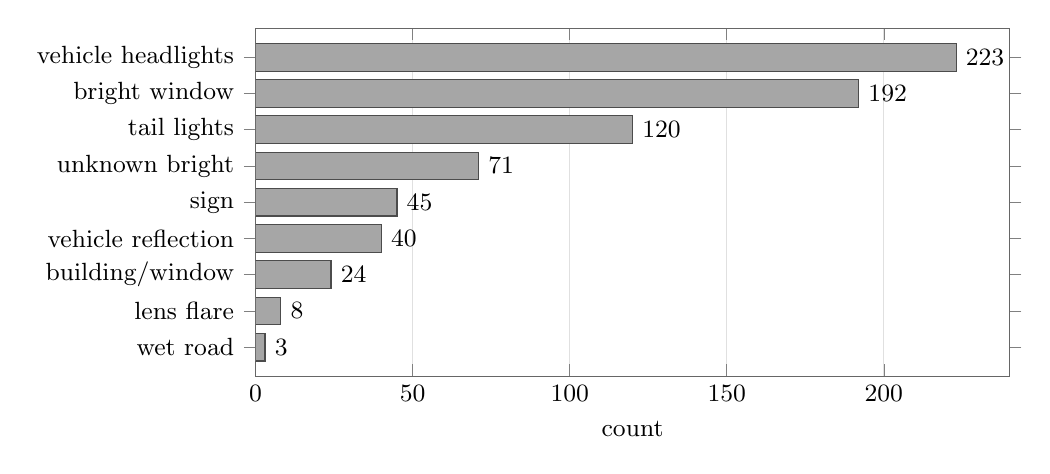
\begin{tikzpicture}
\begin{axis}[
    xbar,
    width=0.92\linewidth,
    height=6.0cm,
    xmin=0,
    xmax=240,
    y dir=reverse,
    symbolic y coords={vehicle headlights,bright window,tail lights,unknown bright,sign,vehicle reflection,building/window,lens flare,wet road},
    ytick=data,
    xtick={0,50,100,150,200},
    xlabel={count},
    tick label style={font=\small},
    label style={font=\small},
    nodes near coords,
    every node near coord/.append style={font=\small},
    axis line style={black!60},
    xmajorgrids,
    grid style={black!12},
]
\addplot[fill=black!35,draw=black!70] coordinates {
    (223,vehicle headlights)
    (192,bright window)
    (120,tail lights)
    (71,unknown bright)
    (45,sign)
    (40,vehicle reflection)
    (24,building/window)
    (8,lens flare)
    (3,wet road)
};
\end{axis}
\end{tikzpicture}
\caption{Confounder types and counts. The dataset contains a variety of bright confounders that could be mistaken for streetlights.}
\end{figure}

\section{Representation-Level Shift Is Directly Measurable}

\begin{table}[H]
\centering
\caption{Embedding-level shift evidence. Training images and deployment video frames were embedded with the detector backbone that is YOLOv26.}
\small
\begin{tabular}{>{\raggedright\arraybackslash}p{0.24\linewidth}>{\raggedright\arraybackslash}p{0.25\linewidth}>{\raggedright\arraybackslash}p{0.41\linewidth}}
\toprule
Test & Observed result & Direct interpretation\\
\midrule
UMAP projection & Train and deployment samples form separated clusters with limited overlap. & The detector backbone maps deployment imagery into a different feature region than training imagery.\\
Wasserstein distance & \(30.17\) between training and deployment embeddings. & Moving one feature distribution onto the other has non-zero transport cost.\\
Domain classifier & \(93.75\%\) train/deployment accuracy. & Latent features contain enough domain information for a classifier to identify the domain far above \(50\%\) chance.\\
\bottomrule
\end{tabular}
\end{table}

\begin{figure}[H]
\centering
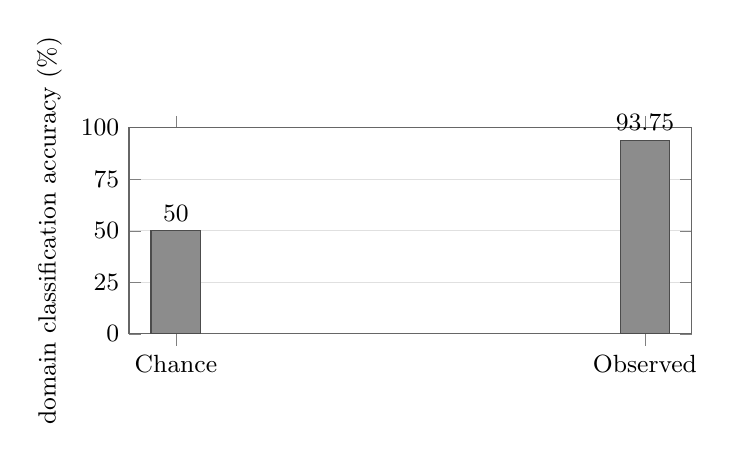
\begin{tikzpicture}
\begin{axis}[
    ybar,
    width=0.72\linewidth,
    height=4.2cm,
    ymin=0,
    ymax=100,
    bar width=18pt,
    symbolic x coords={Chance,Observed},
    xtick=data,
    ylabel={domain classification accuracy (\%)},
    ytick={0,25,50,75,100},
    nodes near coords,
    every node near coord/.append style={font=\small},
    tick label style={font=\small},
    label style={font=\small},
    axis line style={black!60},
    ymajorgrids,
    grid style={black!12},
]
\addplot[fill=black!45,draw=black!70] coordinates {(Chance,50) (Observed,93.75)};
\end{axis}
\end{tikzpicture}
\caption{A domain classifier separates training and deployment embeddings at \(93.75\%\), far above chance. This is direct feature-space evidence of deployment shift.}
\end{figure}

\textbf{Interpretation.}
We see the same conclusion in three independent tests: neighborhood geometry, transport discrepancy, and domain predictability. Since the split appears in learned backbone embeddings, An argument can be made for a representation-level deployment shift.

\section{Literature Shows This Is A General Problem}

\begin{table}[H]
\centering
\caption{Local literature-review evidence that mobile night-time streetlight detection and measurement face domain shift beyond this dataset.}
\scriptsize
\begin{tabular}{>{\raggedright\arraybackslash}p{0.21\linewidth}>{\raggedright\arraybackslash}p{0.32\linewidth}>{\raggedright\arraybackslash}p{0.39\linewidth}}
\toprule
Evidence type & Local source & What it establishes\\
\midrule
Mobile streetlight auditing & Kumar et al. (2016), \textit{Urban Street Lighting Infrastructure Monitoring Using a Mobile Sensor Platform} & Night drive-by streetlight monitoring is already recognized as a scalable sensing problem requiring lamp identification, geotagging, height estimation, and illumination mapping.\\
Dashcam streetlight detection & Aiymbay et al. (2025), \textit{Applying Computer Vision for the Detection and Analysis of the Condition and Operation of Street Lighting} & Recent work builds a 4,260-frame night-weather dashcam dataset for poles and lamps, showing the detection problem is real but still not equivalent to useful-illumination measurement.\\
Night-time scene perception & Tan et al. (2022), \textit{Night-time Scene Parsing with a Large Real Dataset} & Night scenes contain simultaneous under- and over-exposure. Models designed around day-time assumptions do not transfer cleanly without night-specific data and exposure-aware modeling.\\
Low-light object detection & Du et al. (2024), \textit{Boosting Object Detection with Zero-Shot Day-Night Domain Adaptation} & Detectors trained on well-lit data degrade in low-light target domains, motivating day-night adaptation and illumination-invariant representations.\\
Broad day-night adaptation & Luo et al. (2023), \textit{Similarity Min-Max: Zero-Shot Day-Night Domain Adaptation} & Day-night shift affects multiple high-level vision tasks, including segmentation, recognition, classification, and video action recognition.\\
Phone light measurement limits & Gutierrez-Martinez et al. (2017), \textit{Smartphones as a Light Measurement Tool: Case of Study} & Smartphones can support light sensing only with calibration and accuracy limits. Phone images/sensors are not direct replacements for controlled photometric instruments.\\
\bottomrule
\end{tabular}
\end{table}

\section{Labelled Examples Show Meticulous Operational Annotation}

\begin{figure}[H]
\centering
\begin{tikzpicture}[x=0.00075\linewidth,y=-0.00075\linewidth]
\node[anchor=north west,inner sep=0] at (0,0)
  {\includegraphics[width=0.96\linewidth]{../../../exports/annotations_LLM/batch_002/image_batch/chatgpt_streetlight_measurement_batch_002_100/images/022_seed_streetlight_dataset_test_train_set_1_frame_253_jpg.rf.tEuIvRBsbXLfiaX0MjRc.jpg}};
\filldraw[yellow!80!black,fill opacity=0.18,draw=yellow!60!black,line width=1.1pt] (390,610)--(1175,610)--(1280,720)--(260,720)--cycle;
\draw[green!70!black,line width=1.2pt] (331,350) rectangle (350,368);
\draw[green!70!black,line width=1.2pt] (710,345) rectangle (726,365);
\draw[green!70!black,line width=1.2pt] (725,346) rectangle (742,365);
\draw[green!70!black,line width=1.2pt] (987,314) rectangle (1008,335);
\draw[green!70!black,line width=1.2pt] (1048,335) rectangle (1068,355);
\draw[blue!80!black,line width=1.1pt] (730,370) rectangle (743,455);
\draw[blue!80!black,line width=1.1pt] (1080,350) rectangle (1092,478);
\draw[red!80!black,line width=1.1pt] (665,402) rectangle (736,432);
\draw[red!80!black,line width=1.1pt] (1128,405) rectangle (1195,450);
\draw[red!80!black,line width=1.1pt] (380,615) rectangle (1180,720);
\node[anchor=north west,fill=white,fill opacity=0.80,text opacity=1,font=\small] at (12,12)
{5 lamps, 2 poles, sign/building-light confounders, hood-reflection polygon};
\end{tikzpicture}
\caption{Example A: quiet campus intersection with multiple lamp heads, visible poles, sign/building-light confounders, and a foreground hood-reflection polygon. Green=lamp, blue=pole, red=confounder, yellow=polygon.}
\end{figure}

\begin{figure}[H]
\centering
\begin{tikzpicture}[x=0.00075\linewidth,y=-0.00075\linewidth]
\node[anchor=north west,inner sep=0] at (0,0)
  {\includegraphics[width=0.96\linewidth]{../../../exports/annotations_LLM/batch_002/image_batch/chatgpt_streetlight_measurement_batch_002_100/images/063_mobile_night_video_20250529_2050207_frame_0021.jpg}};
\filldraw[yellow!80!black,fill opacity=0.15,draw=yellow!60!black,line width=1.0pt] (0,560)--(470,355)--(820,355)--(1280,545)--(1280,720)--(0,720)--cycle;
\filldraw[orange!90!black,fill opacity=0.13,draw=orange!80!black,line width=1.0pt] (360,470)--(645,365)--(940,410)--(1280,560)--(1280,720)--(360,720)--cycle;
\draw[green!70!black,line width=1.2pt] (500,346) rectangle (530,375);
\draw[green!70!black,line width=1.2pt] (852,223) rectangle (890,257);
\draw[blue!80!black,line width=1.1pt] (450,355) rectangle (463,548);
\draw[blue!80!black,line width=1.1pt] (806,250) rectangle (822,425);
\draw[red!80!black,line width=1.1pt] (730,540) rectangle (985,665);
\draw[red!80!black,line width=1.1pt] (940,505) rectangle (1005,550);
\draw[red!80!black,line width=1.1pt] (1055,385) rectangle (1135,455);
\node[anchor=north west,fill=white,fill opacity=0.80,text opacity=1,font=\small] at (12,12)
{2 lamp/pole pairs, 3 bright confounders, road + lit-area polygons};
\end{tikzpicture}
\caption{Example B: separate lamp/pole tracks are labelled alongside vehicle headlights, a reflective sign, public road surface, and approximate lit area.}
\end{figure}

\begin{figure}[H]
\centering
\begin{tikzpicture}[x=0.00075\linewidth,y=-0.00075\linewidth]
\node[anchor=north west,inner sep=0] at (0,0)
  {\includegraphics[width=0.96\linewidth]{../../../exports/annotations_LLM/batch_003/image_batch/chatgpt_streetlight_measurement_batch_003_100/images/019_mobile_night_video_56165151815_frame_0015.jpg}};
\draw[green!70!black,line width=1.2pt] (969,46) rectangle (991,68);
\draw[green!70!black,line width=1.2pt] (800,211) rectangle (815,228);
\draw[green!70!black,line width=1.2pt] (535,210) rectangle (550,226);
\draw[green!70!black,line width=1.2pt] (483,275) rectangle (498,289);
\draw[blue!80!black,line width=1.1pt] (1058,78) rectangle (1072,370);
\draw[blue!80!black,line width=1.1pt] (836,224) rectangle (850,390);
\draw[red!80!black,line width=1.1pt] (0,190) rectangle (195,327);
\draw[red!80!black,line width=1.1pt] (590,530) rectangle (820,590);
\draw[red!80!black,line width=1.1pt] (890,395) rectangle (940,430);
\draw[red!80!black,line width=1.1pt] (934,380) rectangle (1280,620);
\draw[red!80!black,line width=1.1pt] (0,460) rectangle (194,720);
\draw[red!80!black,line width=1.1pt] (400,385) rectangle (475,430);
\node[anchor=north west,fill=white,fill opacity=0.80,text opacity=1,font=\small] at (12,12)
{4 lamps, 2 poles, 6 traffic/shopfront confounders};
\end{tikzpicture}
\caption{Example C: busy arterial scene with streetlight tracks separated from vehicle lights, auto-rickshaw reflections, and shopfront/window bright sources.}
\end{figure}

\begin{figure}[H]
\centering
\begin{tikzpicture}[x=0.00075\linewidth,y=-0.00075\linewidth]
\node[anchor=north west,inner sep=0] at (0,0)
  {\includegraphics[width=0.96\linewidth]{../../../exports/annotations_LLM/batch_001/image_batch/chatgpt_streetlight_measurement_batch_001_100/images/098_mobile_night_video_56165151815_frame_0025.jpg}};
\draw[green!70!black,line width=1.2pt] (553,106) rectangle (569,125);
\draw[green!70!black,line width=1.2pt] (571,262) rectangle (586,280);
\draw[green!70!black,line width=1.2pt] (880,210) rectangle (898,230);
\draw[blue!80!black,line width=1.1pt] (497,125) rectangle (512,472);
\draw[blue!80!black,line width=1.1pt] (555,280) rectangle (568,390);
\draw[blue!80!black,line width=1.1pt] (903,230) rectangle (916,462);
\draw[red!80!black,line width=1.1pt] (785,452) rectangle (925,551);
\draw[red!80!black,line width=1.1pt] (1018,320) rectangle (1278,421);
\draw[red!80!black,line width=1.1pt] (726,422) rectangle (748,446);
\draw[red!80!black,line width=1.1pt] (388,407) rectangle (572,585);
\node[anchor=north west,fill=white,fill opacity=0.80,text opacity=1,font=\small] at (12,12)
{3 lamp/pole pairs, taillights, vehicle windows, headlights, reflection};
\end{tikzpicture}
\caption{Example D: multi-lane traffic scene with pole-linked lamps labelled separately from taillights, vehicle windows, headlights, and reflections.}
\end{figure}

\textbf{Interpretation.}
These four examples show quiet-campus, glare/road-surface, busy-arterial, and multi-lane traffic cases. The baseline labels already encode the operational context needed by the deployed system. The remaining failures therefore test whether the representation and downstream operator use this structure correctly, not whether labels were merely absent.

\section{Diverse Labelling Does Not Guarantee Operational Accuracy}

\begin{table}[H]
\centering
\caption{End-to-end deployment shift despite the presence of diverse baseline labels.}
\scriptsize
\begin{tabular}{lrrrrrr}
\toprule
Scene & Labelled lamps & Detector tracks & Extra detections & Unknown reports & Review flags & Invalid reports\\
\midrule
Quiet residential & 2 & 6 & 4 & 6 & 6 & 6\\
Heavy glare traffic & 1 & 8 & 7 & 8 & 8 & 8\\
Busy arterial & 1 & 5 & 4 & 5 & 4 & 5\\
Clean negative & 0 & 6 & 6 & 6 & 4 & 6\\
\bottomrule
\end{tabular}
\end{table}

\begin{figure}[H]
\centering
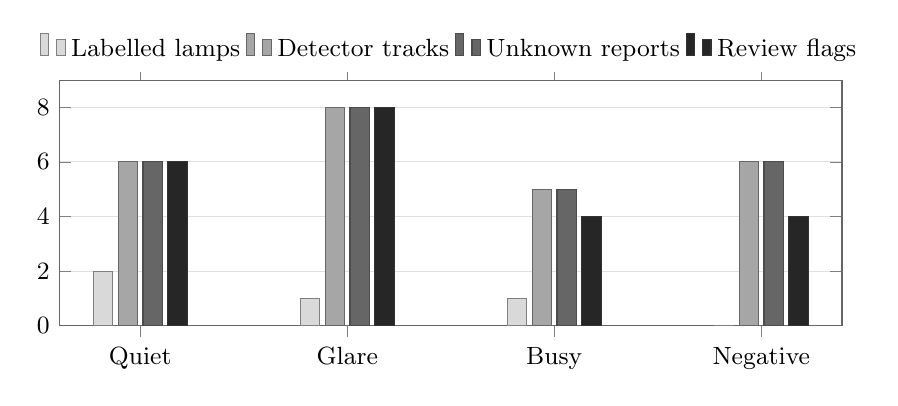
\begin{tikzpicture}
\begin{axis}[
    ybar,
    width=0.95\linewidth,
    height=4.7cm,
    ymin=0,
    ymax=9,
    bar width=7pt,
    symbolic x coords={Quiet,Glare,Busy,Negative},
    xtick=data,
    ytick={0,2,4,6,8},
    enlarge x limits=0.13,
    tick label style={font=\small},
    legend style={font=\small,draw=none,at={(0.5,1.03)},anchor=south,legend columns=4},
    axis line style={black!60},
    ymajorgrids,
    grid style={black!12},
]
\addplot[fill=black!15,draw=black!50] coordinates {(Quiet,2) (Glare,1) (Busy,1) (Negative,0)};
\addplot[fill=black!35,draw=black!60] coordinates {(Quiet,6) (Glare,8) (Busy,5) (Negative,6)};
\addplot[fill=black!60,draw=black!70] coordinates {(Quiet,6) (Glare,8) (Busy,5) (Negative,6)};
\addplot[fill=black!85,draw=black!80] coordinates {(Quiet,6) (Glare,8) (Busy,4) (Negative,4)};
\legend{Labelled lamps,Detector tracks,Unknown reports,Review flags}
\end{axis}
\end{tikzpicture}
\caption{Diverse labels do not prevent operational amplification: shifted or negative inputs produce excess detector tracks and unusable downstream reports.}
\end{figure}

\textbf{Interpretation.}
The heavy-glare scene has one annotated lamp but yields eight detector tracks and eight unknown/invalid reports. The busy-arterial scene has one annotated lamp but yields five detector tracks and five invalid reports, nearly matching the clean-negative failure load. This is direct evidence that label diversity alone does not imply deployed operational accuracy.

\section{Measurement Error Depends on Detection Error}

\begin{figure}[H]
\centering
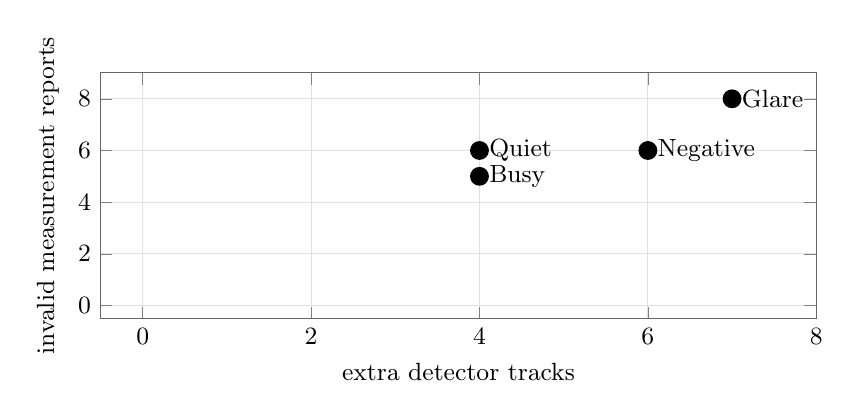
\begin{tikzpicture}
\begin{axis}[
    width=0.88\linewidth,
    height=4.7cm,
    xmin=-0.5,
    xmax=8,
    ymin=-0.5,
    ymax=9,
    xlabel={extra detector tracks},
    ylabel={invalid measurement reports},
    xtick={0,2,4,6,8},
    ytick={0,2,4,6,8},
    tick label style={font=\small},
    label style={font=\small},
    axis line style={black!60},
    grid=major,
    grid style={black!12},
]
\addplot[only marks,mark=*,mark size=3.2pt] coordinates {(4,6) (7,8) (4,5) (6,6)};
\node[anchor=west,font=\small] at (axis cs:4,6) {Quiet};
\node[anchor=west,font=\small] at (axis cs:7,8) {Glare};
\node[anchor=west,font=\small] at (axis cs:4,5) {Busy};
\node[anchor=west,font=\small] at (axis cs:6,6) {Negative};
\end{axis}
\end{tikzpicture}
\caption{Extra detector tracks propagate into invalid measurement reports. Measurement is not independent of detection. False or duplicated detections become false audit objects.}
\end{figure}

\textbf{Interpretation.}
The measurement stage consumes detector tracks. Quiet, glare, busy-arterial, and clean-negative cases have invalid-per-track rate 1.00. The manual-review-per-track rate is 1.00 for quiet/glare, .80 for busy, and .67 for clean negative. When deployment shift creates extra detections, the measurement block emits extra invalid, unknown, or manual-review reports. This proves that the downstream operator depends on the representation and detection geometry.

\section{Conclusive Argument}
Taken together, the evidence closes the main loopholes. We have diverse baseline labels, direct representation-level shift, external literature showing that night/mobile shift is a general problem, and downstream reports showing that extra detections become invalid operational measurements. The conclusion is therefore specific: representation learning must preserve directions that change downstream validity and collapse only directions that are operationally irrelevant.

\end{document}
